\clearpage
\section{}

\subsection{Show that the alloys chosen are not ideal}

Lattice parameters:
\begin{align}
  \label{eq:01}
    \begin{split}
        a_\gamma &= 3.523 + 0.179 Al + 0.700Ta + 0.110 Cr + 0.444W+ 0.441 Re \\
        & + 0.478Mo + 0.096 Co \\
        a_{\gamma'} &= 3.558 + 0.500Ta ¡ 0.004 Cr + 0.194W+ 0.262 Re + 0.208Mo
    \end{split}
\end{align}

Lattice misfit equation
\begin{align}
  \label{eq:02}
    \delta &= 2\times\left[\dfrac{a_{\gamma'}-a_\gamma}{a_{\gamma'}+a_\gamma}\right]
\end{align}

Using the \textit{One axis} tool in \textit{ThermoCalc} the composition of the different phases of the alloy were calculated. Using these values and equation \ref{eq:01}, the lattice parameter of the $\gamma$ and $\gamma'$ phases were calculated. Then, the lattice misfit, $\delta$, was calculated using \ref{eq:02}. The results obtained are presented in \ref{tab:tab03}:

\begin{table}[h]
    \centering
    \begin{tabular}{rrrrrrrrr}
        \multicolumn{1}{c}{Ni$_\gamma$} & \multicolumn{1}{c}{Al$_\gamma$} & \multicolumn{1}{c}{Ta$_\gamma$} & \multicolumn{1}{c}{Ni$_{\gamma'}$} & \multicolumn{1}{c}{Al$_{\gamma'}$} & \multicolumn{1}{c}{Ta$_{\gamma'}$} & \multicolumn{1}{c}{$a_\gamma$} & \multicolumn{1}{c}{$a_{\gamma'}$} & \multicolumn{1}{c}{$\delta$} \\ \hline \hline
        0.8633 & 0.1317 & 0.0050 & 0.7842 & 0.1908 & 0.0250 & 3.5501 & 3.5705 & 0.0057 \\0.8721 & 0.1156 & 0.0123 & 0.7909 & 0.1732 & 0.0359 & 3.5523 & 3.5760 & 0.0066 \\0.8789 & 0.0979 & 0.0232 & 0.7954 & 0.1590 & 0.0456 & 3.5568 & 3.5808 & 0.0067 \\0.8826 & 0.0809 & 0.0365 & 0.7978 & 0.1477 & 0.0545 & 3.5630 & 3.5853 & 0.0062 \\0.8830 & 0.0661 & 0.0509 & 0.7982 & 0.1388 & 0.0630 & 3.5705 & 3.5895 & 0.0053 \\0.8803 & 0.0541 & 0.0655 & 0.7970 & 0.1315 & 0.0715 & 3.5786 & 3.5937 & 0.0042 \\0.8751 & 0.0448 & 0.0800 & 0.7947 & 0.1253 & 0.0800 & 3.5870 & 3.5980 & 0.0030 \\0.8696 & 0.0391 & 0.0913 & 0.7922 & 0.1210 & 0.0868 & 3.5939 & 3.6014 & 0.0021 \\0.8696 & 0.0391 & 0.0913 & 0.7922 & 0.1210 & 0.0868 & 3.5939 & 3.6014 & 0.0021 \\0.8696 & 0.0391 & 0.0913 & 0.7922 & 0.1210 & 0.0868 & 3.5939 & 3.6014 & 0.0021 \\0.8696 & 0.0391 & 0.0913 & 0.7922 & 0.1210 & 0.0868 & 3.5939 & 3.6014 & 0.0021 \\0.8696 & 0.0391 & 0.0913 & 0.7922 & 0.1210 & 0.0868 & 3.5939 & 3.6014 & 0.0021 \\0.8633 & 0.1317 & 0.0050 & 0.7842 & 0.1908 & 0.0250 & 3.5501 & 3.5705 & 0.0057 \\0.8547 & 0.1439 & 0.0013 & 0.7763 & 0.2108 & 0.0129 & 3.5497 & 3.5644 & 0.0041 \\0.8485 & 0.1515 & 0.0000 & 0.7685 & 0.2315 & 0.0000 & 3.5501 & 3.5580 & 0.0022
    \end{tabular}
    \caption{Lattice misfit, $\delta$, calculated for the Ni-Al-Ta alloy using the compositions (molar fractions) of the elements present in $\gamma$ and $\gamma'$ phases obtained using\textit{ThermoCalc} \citep{thermocalc}. The calculations of $a_\gamma$, $a_{\gamma´}$ and $\delta$ were performed in Python \citep{mygit}}
    \label{tab:tab03}
\end{table}

From table \ref{tab:tab03} it can be seen that the values of $\delta$ are not equal to zero, which can indicate that the alloy is not ideal for the different compositions.

\newpage
\subsection{With additions of Cr, W, Re, Mo or mixture, find alloy for which the lattice misfit is close to zero}

The values of the lattice misfit for both $\gamma$ and $\gamma'$ phases were calculated using the molar fractions of the $\gamma$ and $\gamma'$ phases of different alloys of Ni-Al-Ta-X, where X is Cr, Mo, Re and W, obtained from a \textit{ThermoCalc} calculations and equations \ref{eq:01} and \ref{eq:02}. The results obtained are presented in tables \ref{tab:tab04}, ,\ref{tab:tab05}, \ref{tab:tab06} and \ref{tab:tab07} in the Appendix \ref{appendix}.

From the values of lattice misfit obtained for each alloy, the minimum value was extracted in order to know which composition gives a lattice misfit closer to zero, the results are presented in table \ref{tab:tab08}:

\begin{table}[H]
  \centering
  \begin{tabular}{rrrrrrrrrrr}
    \multicolumn{1}{c}{Ni$_\gamma$} & \multicolumn{1}{c}{Al$_\gamma$} & \multicolumn{1}{c}{Ta$_\gamma$} & \multicolumn{1}{c}{Cr$_\gamma$} & \multicolumn{1}{c}{Ni$_{\gamma'}$} & \multicolumn{1}{c}{Al$_{\gamma'}$} & \multicolumn{1}{c}{Ta$_{\gamma'}$} & \multicolumn{1}{c}{Cr$_{\gamma'}$} & \multicolumn{1}{c}{a$_\gamma$} & \multicolumn{1}{c}{a$_{\gamma'}$} & \multicolumn{1}{c}{$\delta$} \\ \hline \hline
    0.7434 & 0.0862 & 0.0077 & 0.1627 & 0.7528 & 0.1741 & 0.0347 & 0.0384 & 3.5617 & 3.5752 & 0.0038 \\\\
   \multicolumn{1}{c}{Ni$_\gamma$} & \multicolumn{1}{c}{Al$_\gamma$} & \multicolumn{1}{c}{Ta$_\gamma$} & \multicolumn{1}{c}{Mo$_\gamma$} & \multicolumn{1}{c}{Ni$_{\gamma'}$} & \multicolumn{1}{c}{Al$_{\gamma'}$} & \multicolumn{1}{c}{Ta$_{\gamma'}$} & \multicolumn{1}{c}{Mo$_{\gamma'}$} & \multicolumn{1}{c}{$a_\gamma$} & \multicolumn{1}{c}{$a_{\gamma'}$} & \multicolumn{1}{c}{$\delta$} \\ \hline \hline
   0.8430 & 0.0843 & 0.0196 & 0.0530 & 0.7731 & 0.1641 & 0.0307 & 0.0320 & 3.5772 & 3.5734 & 0.0011 \\\\
   \multicolumn{1}{c}{Ni$_\gamma$} & \multicolumn{1}{c}{Al$_\gamma$} & \multicolumn{1}{c}{Ta$_\gamma$} & \multicolumn{1}{c}{Re$_\gamma$} & \multicolumn{1}{c}{Ni$_{\gamma'}$} & \multicolumn{1}{c}{Al$_{\gamma'}$} & \multicolumn{1}{c}{Ta$_{\gamma'}$} & \multicolumn{1}{c}{Re$_{\gamma'}$} & \multicolumn{1}{c}{a$_\gamma$} & \multicolumn{1}{c}{a$_{\gamma'}$} & \multicolumn{1}{c}{$\delta$} \\ \hline \hline
   0.8303 & 0.1157 & 0.0087 & 0.0453 & 0.7790 & 0.1798 & 0.0340 & 0.0072 & 3.5698 & 3.5769 & 0.0020 \\\\
   \multicolumn{1}{c}{Ni$_\gamma$} & \multicolumn{1}{c}{Al$_\gamma$} & \multicolumn{1}{c}{Ta$_\gamma$} & \multicolumn{1}{c}{W$_\gamma$} & \multicolumn{1}{c}{Ni$_{\gamma'}$} & \multicolumn{1}{c}{Al$_{\gamma'}$} & \multicolumn{1}{c}{Ta$_{\gamma'}$} & \multicolumn{1}{c}{W$_{\gamma'}$} & \multicolumn{1}{c}{a$_\gamma$} & \multicolumn{1}{c}{a$_{\gamma'}$} & \multicolumn{1}{c}{$\delta$} \\ \hline \hline
   0.8711 & 0.0797 & 0.0199 & 0.0293 & 0.7871 & 0.1588 & 0.0300 & 0.0241 & 3.5642 & 3.5777 & 0.0038
  \end{tabular}
  \caption{Minimum values of lattice misfit, $\delta$, for each alloy calculated using Python \citep{mygit}}
  \label{tab:tab08}
\end{table}

From the values presented in table \ref{tab:tab08}, the minimum value of all the alloys was extracted, which is shown in table \ref{tab:tab09}, with a misfit value of $0.0011$, being the closet value for all the alloys.

\begin{table}[h]
  \begin{tabular}{rrrrrrrrrrrrrrrrr}
    \multicolumn{1}{c}{Ni$_\gamma$} & \multicolumn{1}{c}{Al$_\gamma$} & \multicolumn{1}{c}{Ta$_\gamma$} & \multicolumn{1}{c}{Mo$_\gamma$} & \multicolumn{1}{c}{Ni$_{\gamma'}$} & \multicolumn{1}{c}{Al$_{\gamma'}$} & \multicolumn{1}{c}{Ta$_{\gamma'}$} & \multicolumn{1}{c}{Mo$_{\gamma'}$} & \multicolumn{1}{c}{$a_\gamma$} & \multicolumn{1}{c}{$a_{\gamma'}$} & \multicolumn{1}{c}{$\delta$} \\ \hline \hline
    0.8430 & 0.0843 & 0.0196 & 0.0530 & 0.7731 & 0.1641 & 0.0307 & 0.0320 & 3.5772 & 3.5734 & 0.0011
  \end{tabular}
  \caption{Minim value of lattice misfit from all alloys, corresponding to the Ni-Al-Ta-Mo alloy. Table generated using Python \citep{mygit}.}
  \label{tab:tab09}
\end{table}

\newpage
\subsection{Do Cr, W, Re and Mo alter significantly the fraction of $\gamma'$ present?}

Figure \ref{fig:diagram04} shows the graphs of the amount of all phases as a function of the mole percent of Cr, Mo, Re and W, obtained usinig \textit{ThermoCalc}. The red line is the $\gamma'$ composition and as it can be seen in all four plots the behavior of the $\gamma'$ phase line is different with each system. From these plots it can be said that the presence of Cr, W, Re and Mo do have an effect ont he fraction of $\gamma'$ present.


\begin{figure}[H]
  \centering
  \subfloat[Cr\label{fig:cr}]{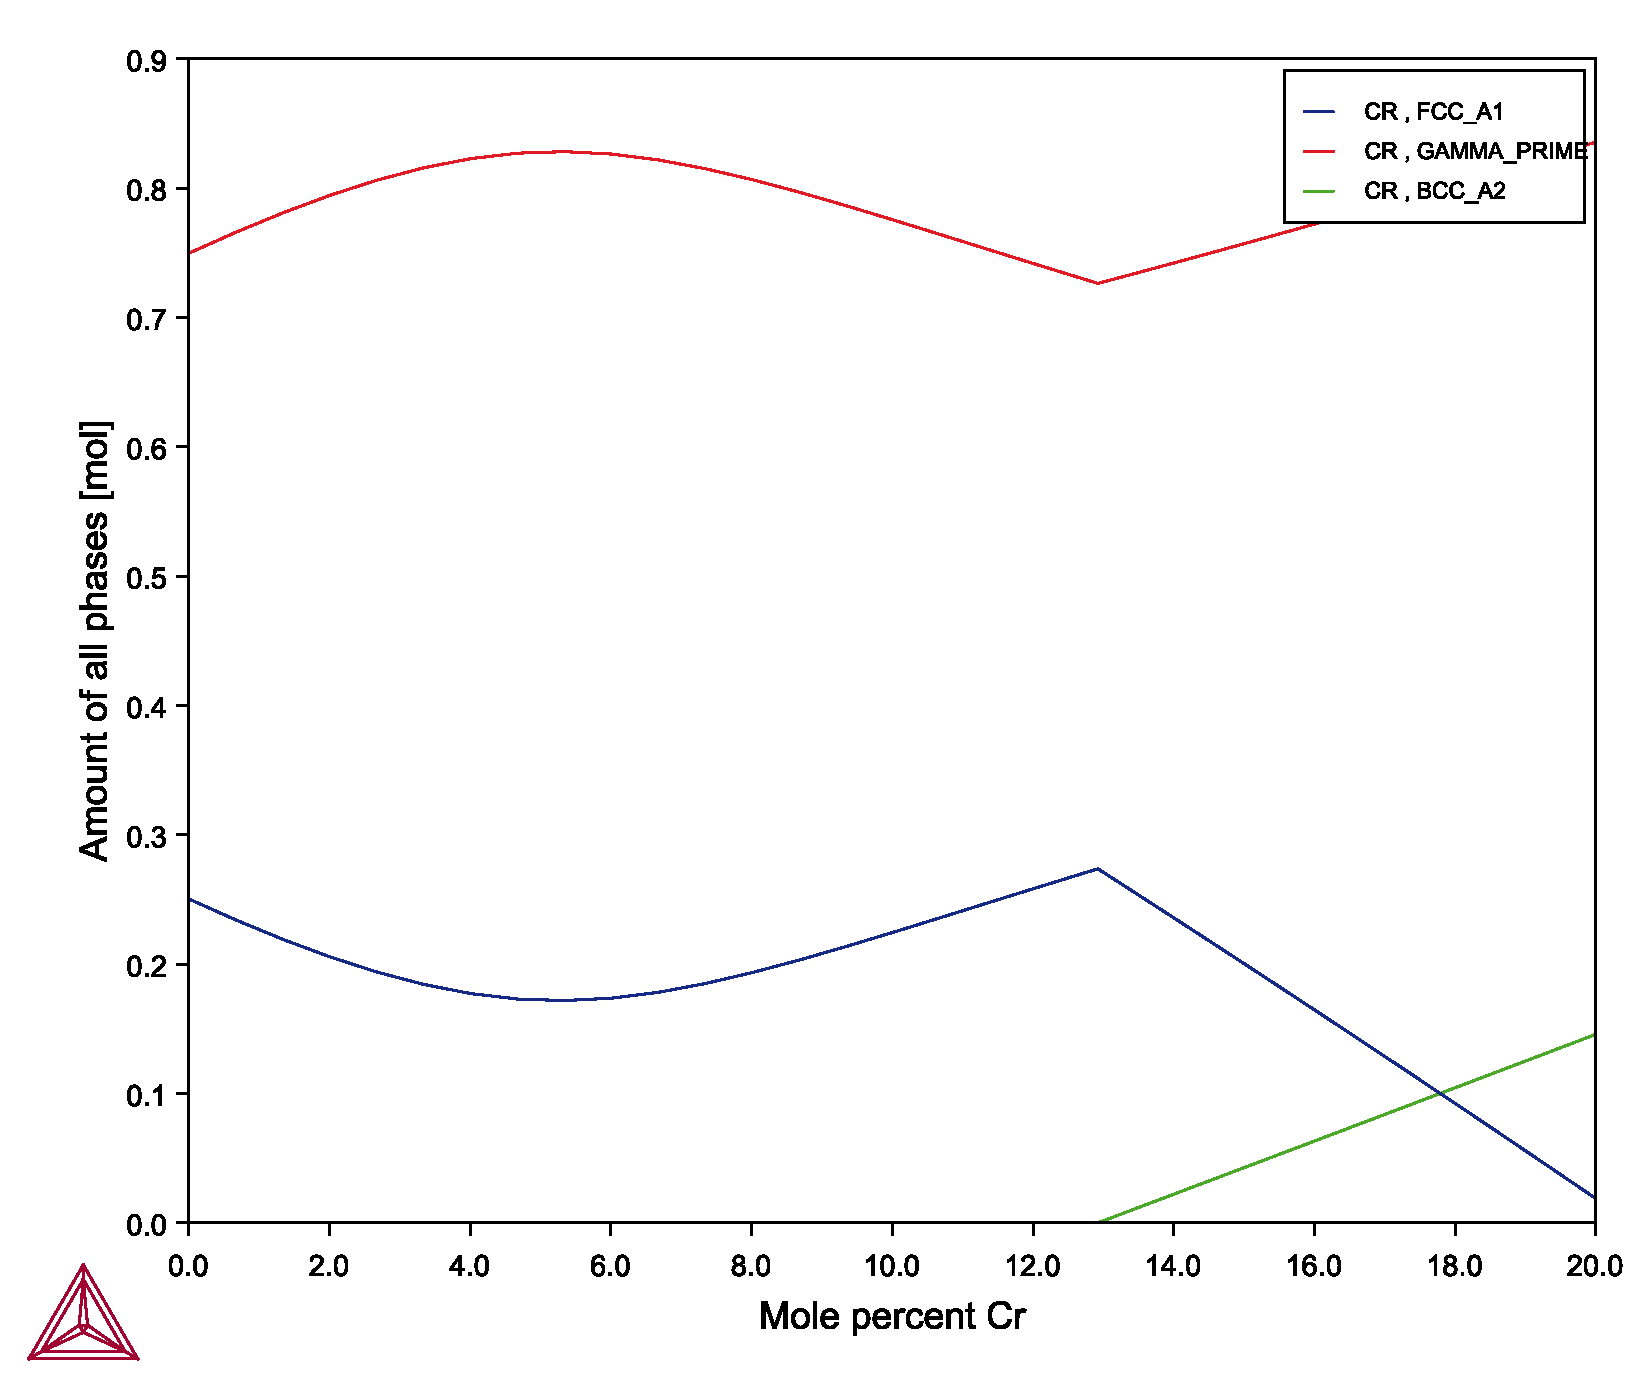
\includegraphics[width=0.5\textwidth]{graficas/Q3_Cr.pdf}}
  \subfloat[Mo\label{fig:mo}]{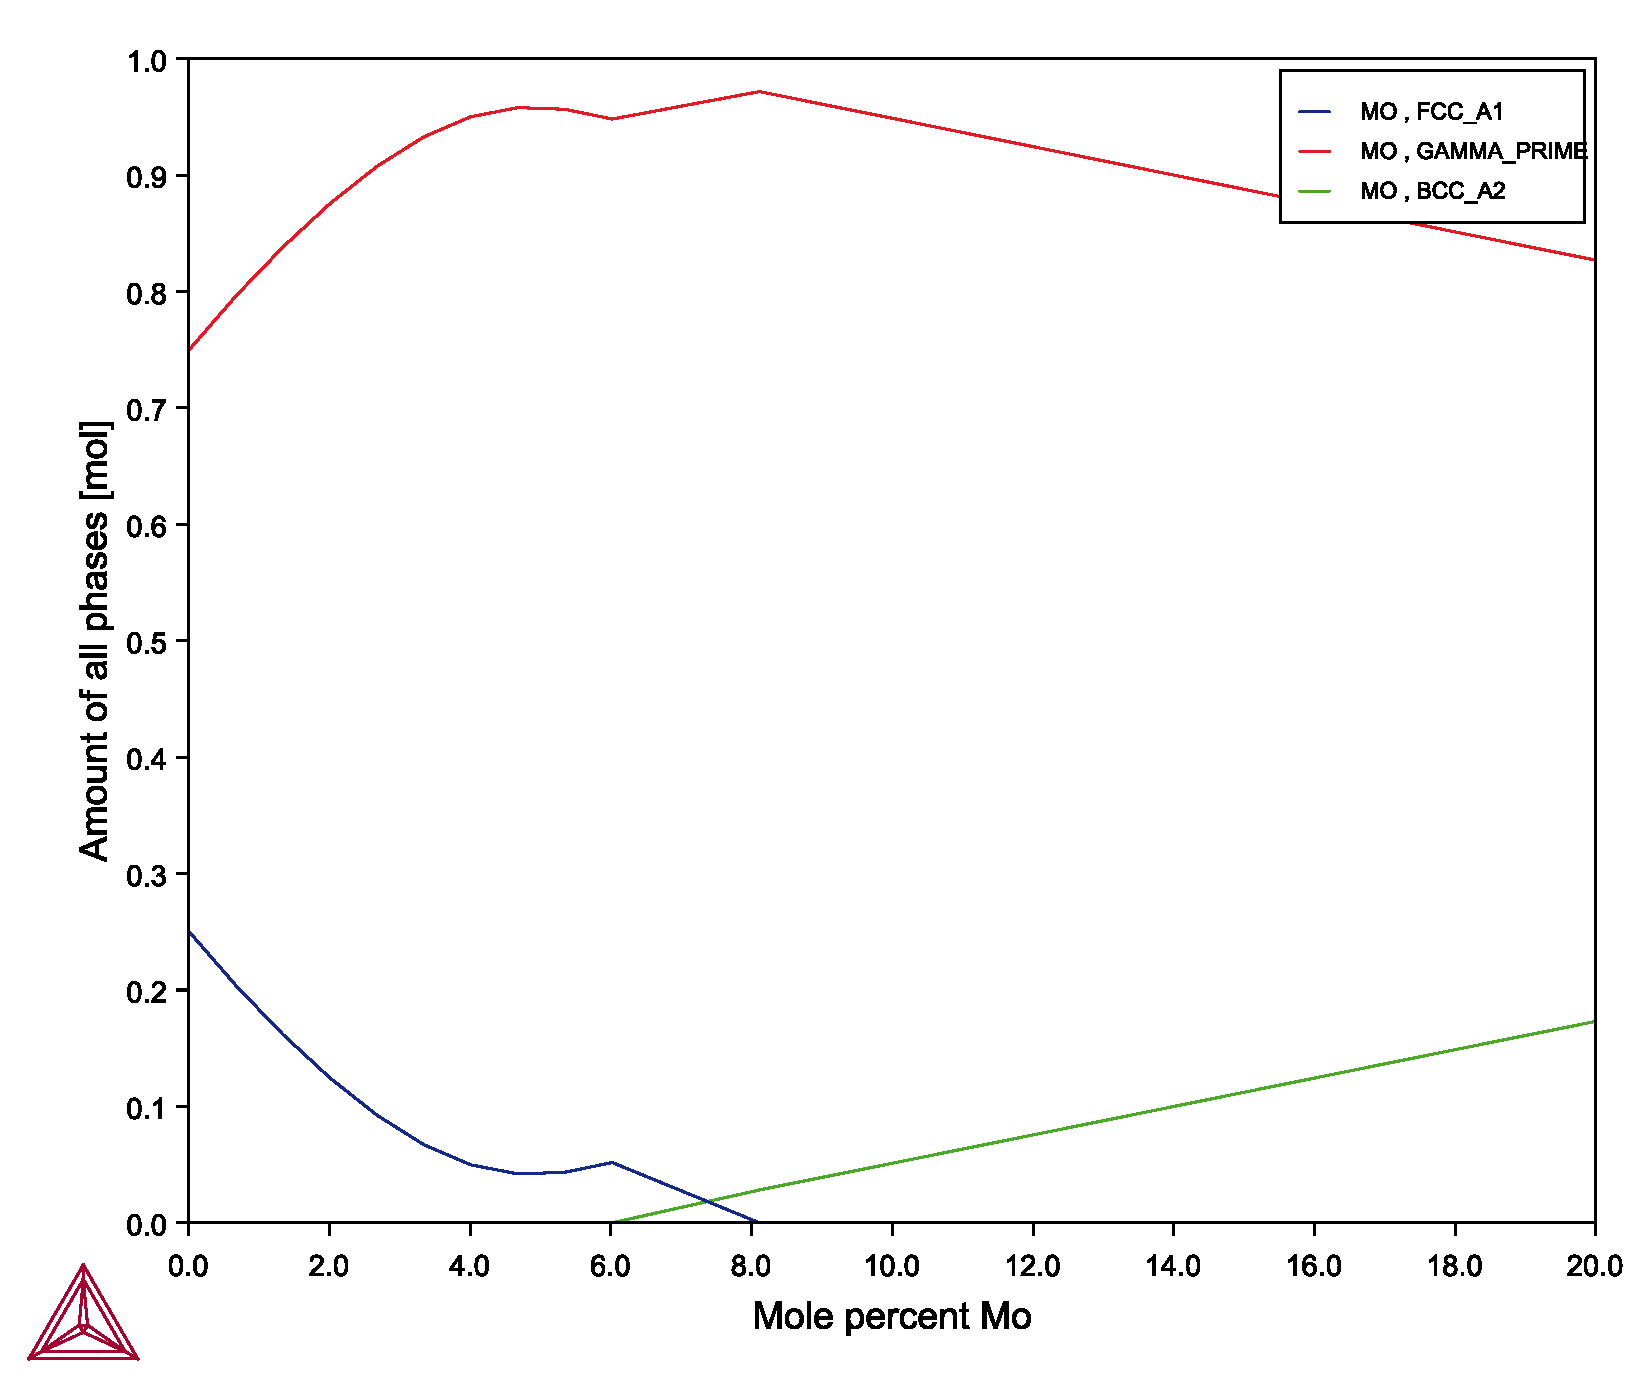
\includegraphics[width=0.5\textwidth]{graficas/Q3_Mo.pdf}} \\
  \subfloat[Re\label{fig:re}]{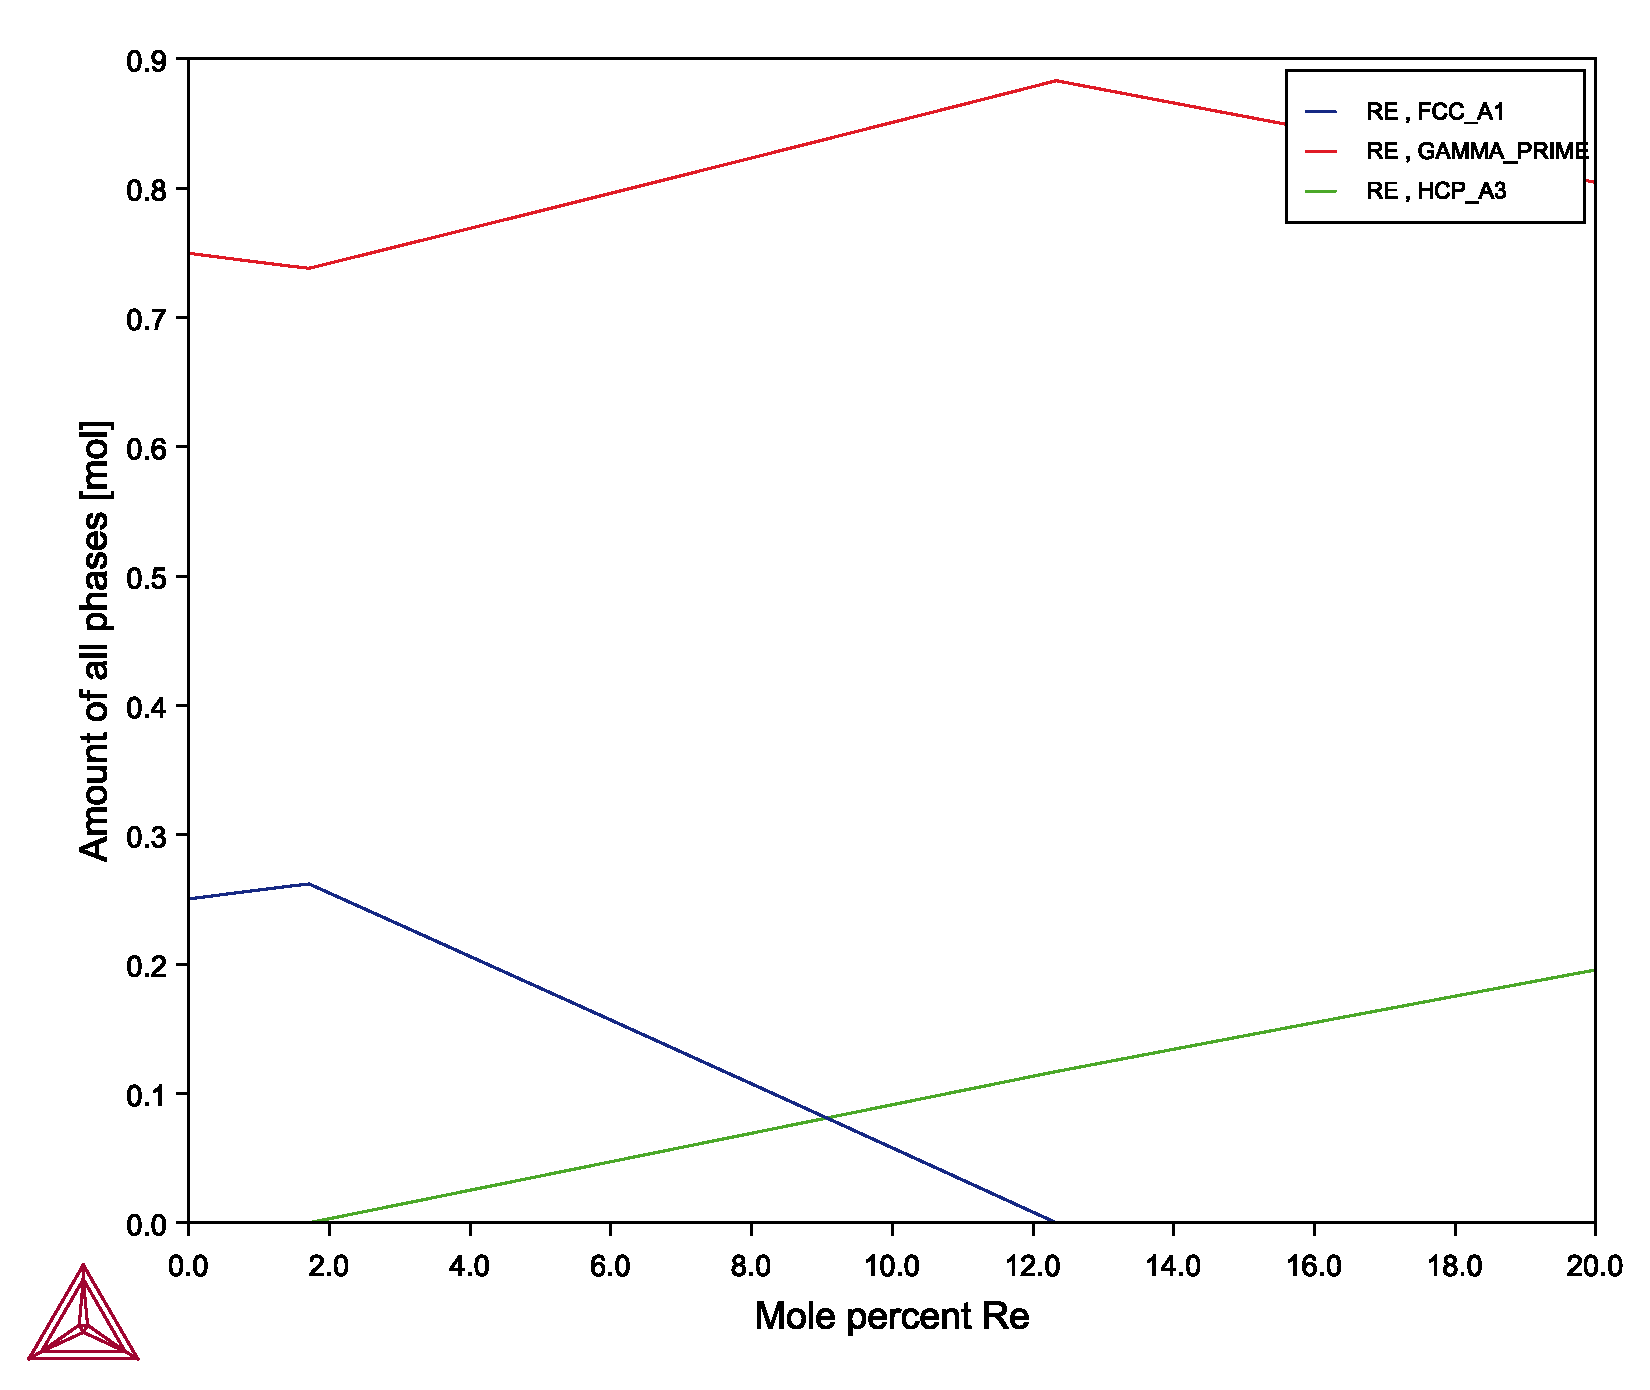
\includegraphics[width=0.5\textwidth]{graficas/Q3_Re.pdf}}
  \subfloat[W\label{fig:w}]{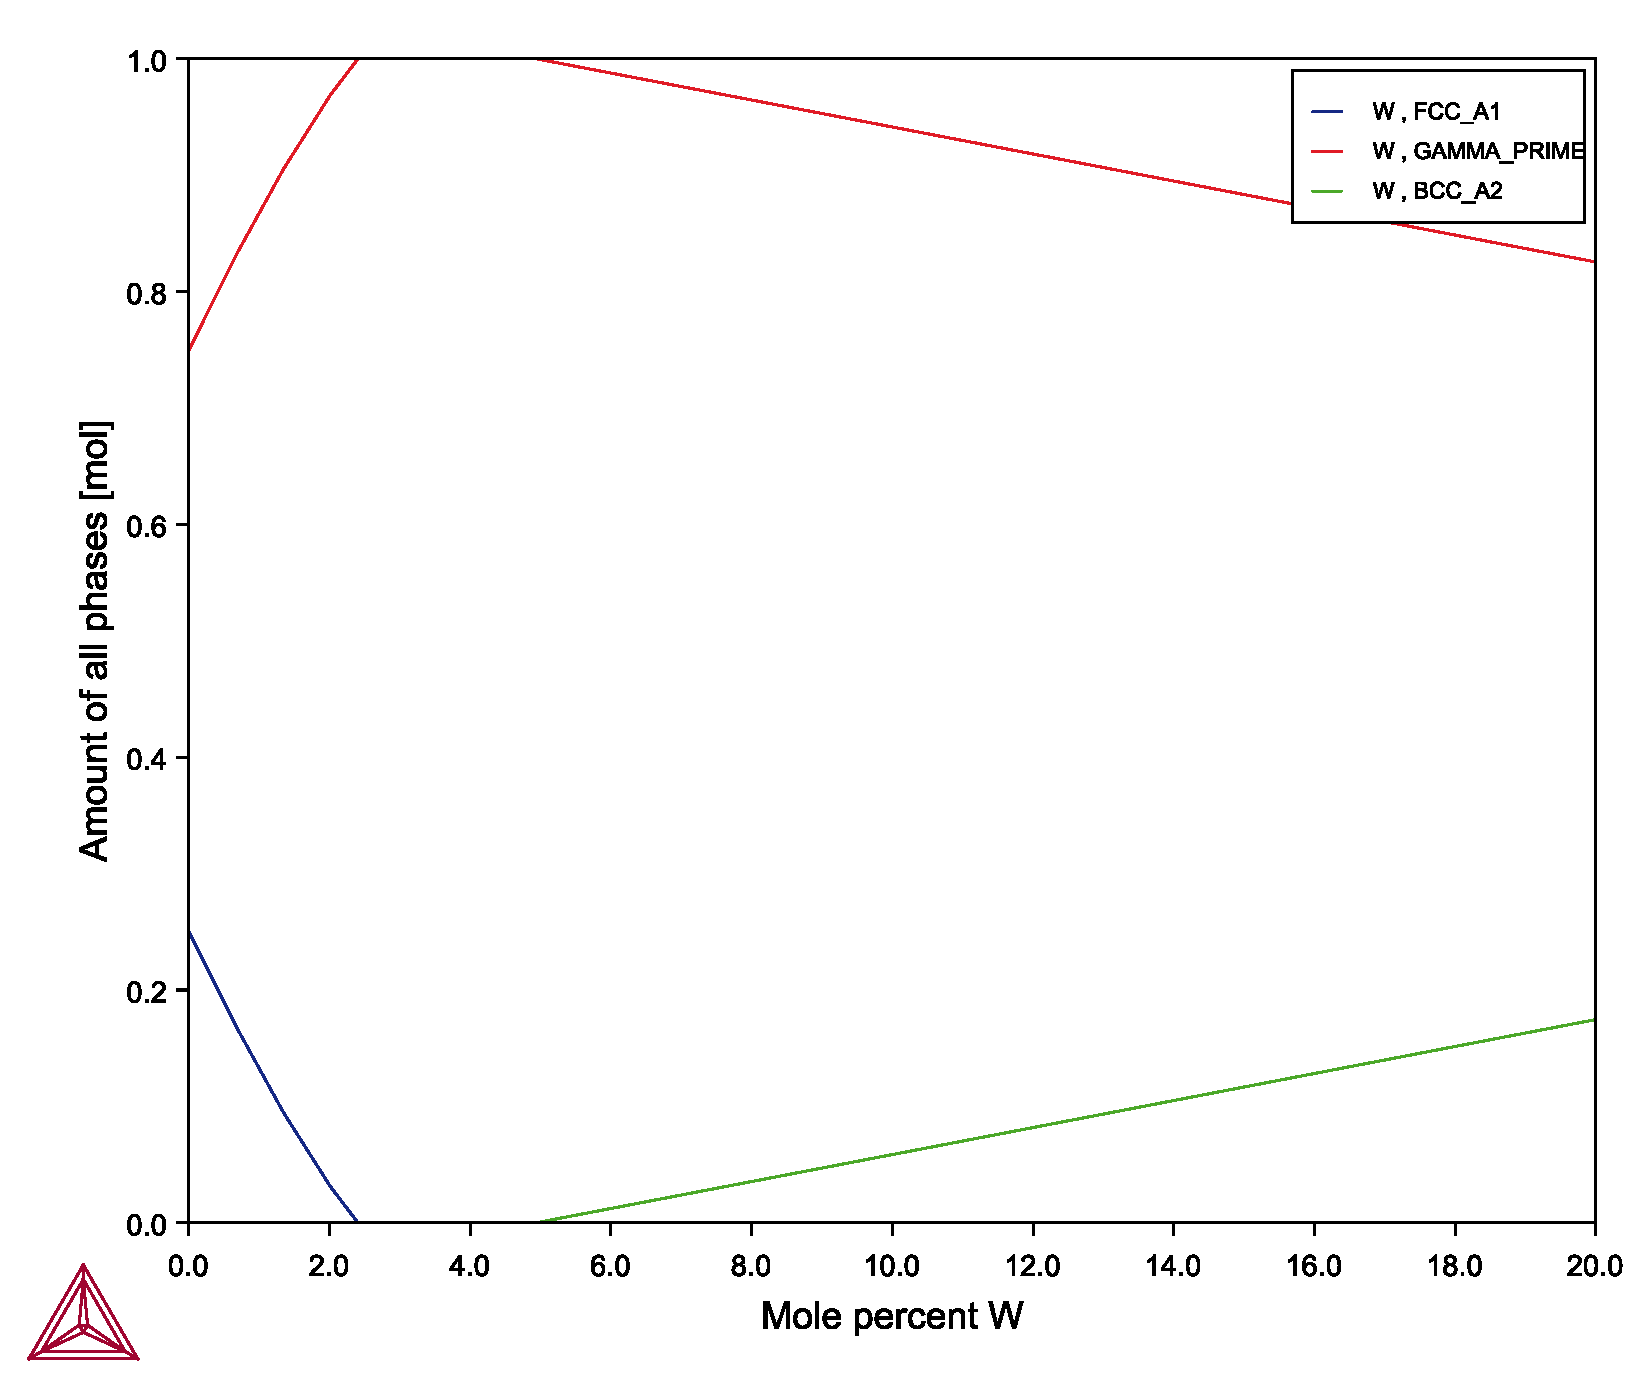
\includegraphics[width=0.5\textwidth]{graficas/Q3_W.pdf}}
  \caption{Amount of phase as function of mole percent of a) Cr, b) Mo, c) Re and d) W generated with \textit{ThermoCalc} \citep{thermocalc}.}
  \label{fig:diagram04}
\end{figure}